\section{Catalan Objects and Dyck Paths}%
\label{sec:catalan_objects}

Dyck paths are one interpretation of the Catalan numbers.
Here, we will instead consider a more general form of Dyck Paths,
which correspond to numbers in the \textit{Catalan Trapezoid}.

A Dyck path can be constructed as a $2n$ step one-dimensional random walk (Figure~\ref{fig:basic_dyck}).
Each step in the walk moves one unit along the positive $x$-axis and one unit up or down the positive $y$-axis.
Given these restrictions, we would obtain a 1D random walk pinned to zero  on both sides.
A Dyck path also has the additional restriction that the $y$-coordinate of any point on the random walk is $\ge 0$.
i.e. the walk is always north of the origin.

The number of possible Dyck paths is the $n^{th}$ Catalan number --
$$C_n = \frac{1}{n+1}\cdot {2n\choose n}$$
We will attempt to support queries to a uniformly random instance of a Dyck path.
Specifically, we will want to answer queries of the form \func{Height}$(i)$,
which returns the position of the path after $i$ steps.

\begin{figure}[htbp]
    \centering
    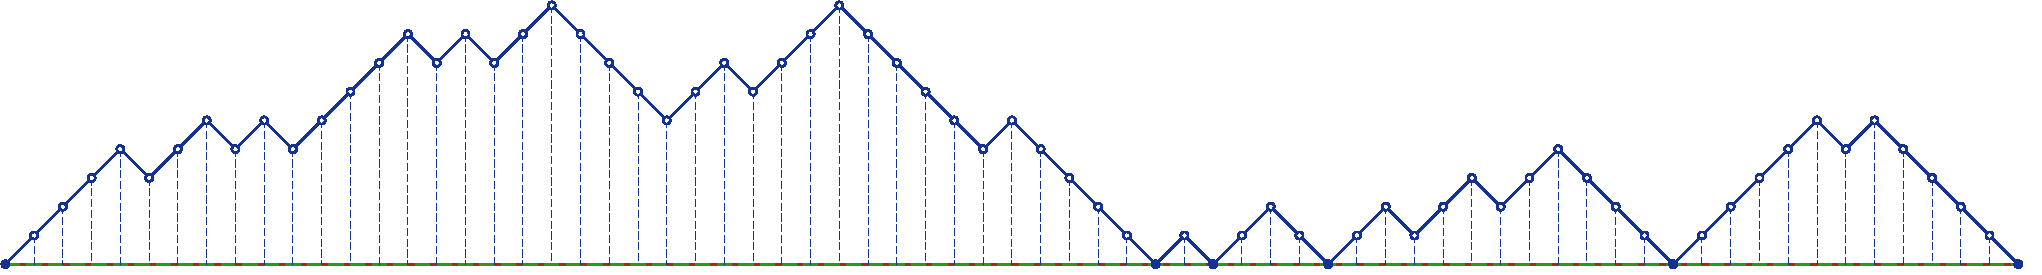
\includegraphics[width=\textwidth]{dyck/basic_dyck_path.pdf}
    \caption{Simple Dyck path with $n = 35$.}
    \label{fig:basic_dyck}
\end{figure}


\subsection{Catalan Trapezoids and Generalized Dyck Paths}
First, we define Catalan trapezoids as presented in \cite{trap}.
Let $C_k(n,m)$ be the $(n,m)^{th}$ entry of the Catalan trapezoid of order $k$,
where $C_1(n,m)$ corresponds to the Catalan triangle.

The interpretation is as follows. Consider a sequence of $n$ up-steps and $m$ down-steps,
such that the sum of any initial sub-string is not less than $1-k$.
This means that we start our Dyck path at a height of $k-1$,
and we are never allowed to cross below zero (Figure~\ref{fig:complex_dyck}).
The total number of such paths is exactly $C_k(n,m)$.
For $k = 1$, we obtain the definition of the simple Dyck path (Figure~\ref{fig:basic_dyck}).

Now, we state a result from \cite{trap} without proof
$$
C_k(n,m)=
\begin{cases}
{n+m}\choose m &0\le m<k\\
{{n+m}\choose{m}} - {{n+m}\choose{m-k}} &k\le m\le n+k-1\\
0 &m>n+k-1
\end{cases}
$$

\begin{figure}[htbp]
    \centering
    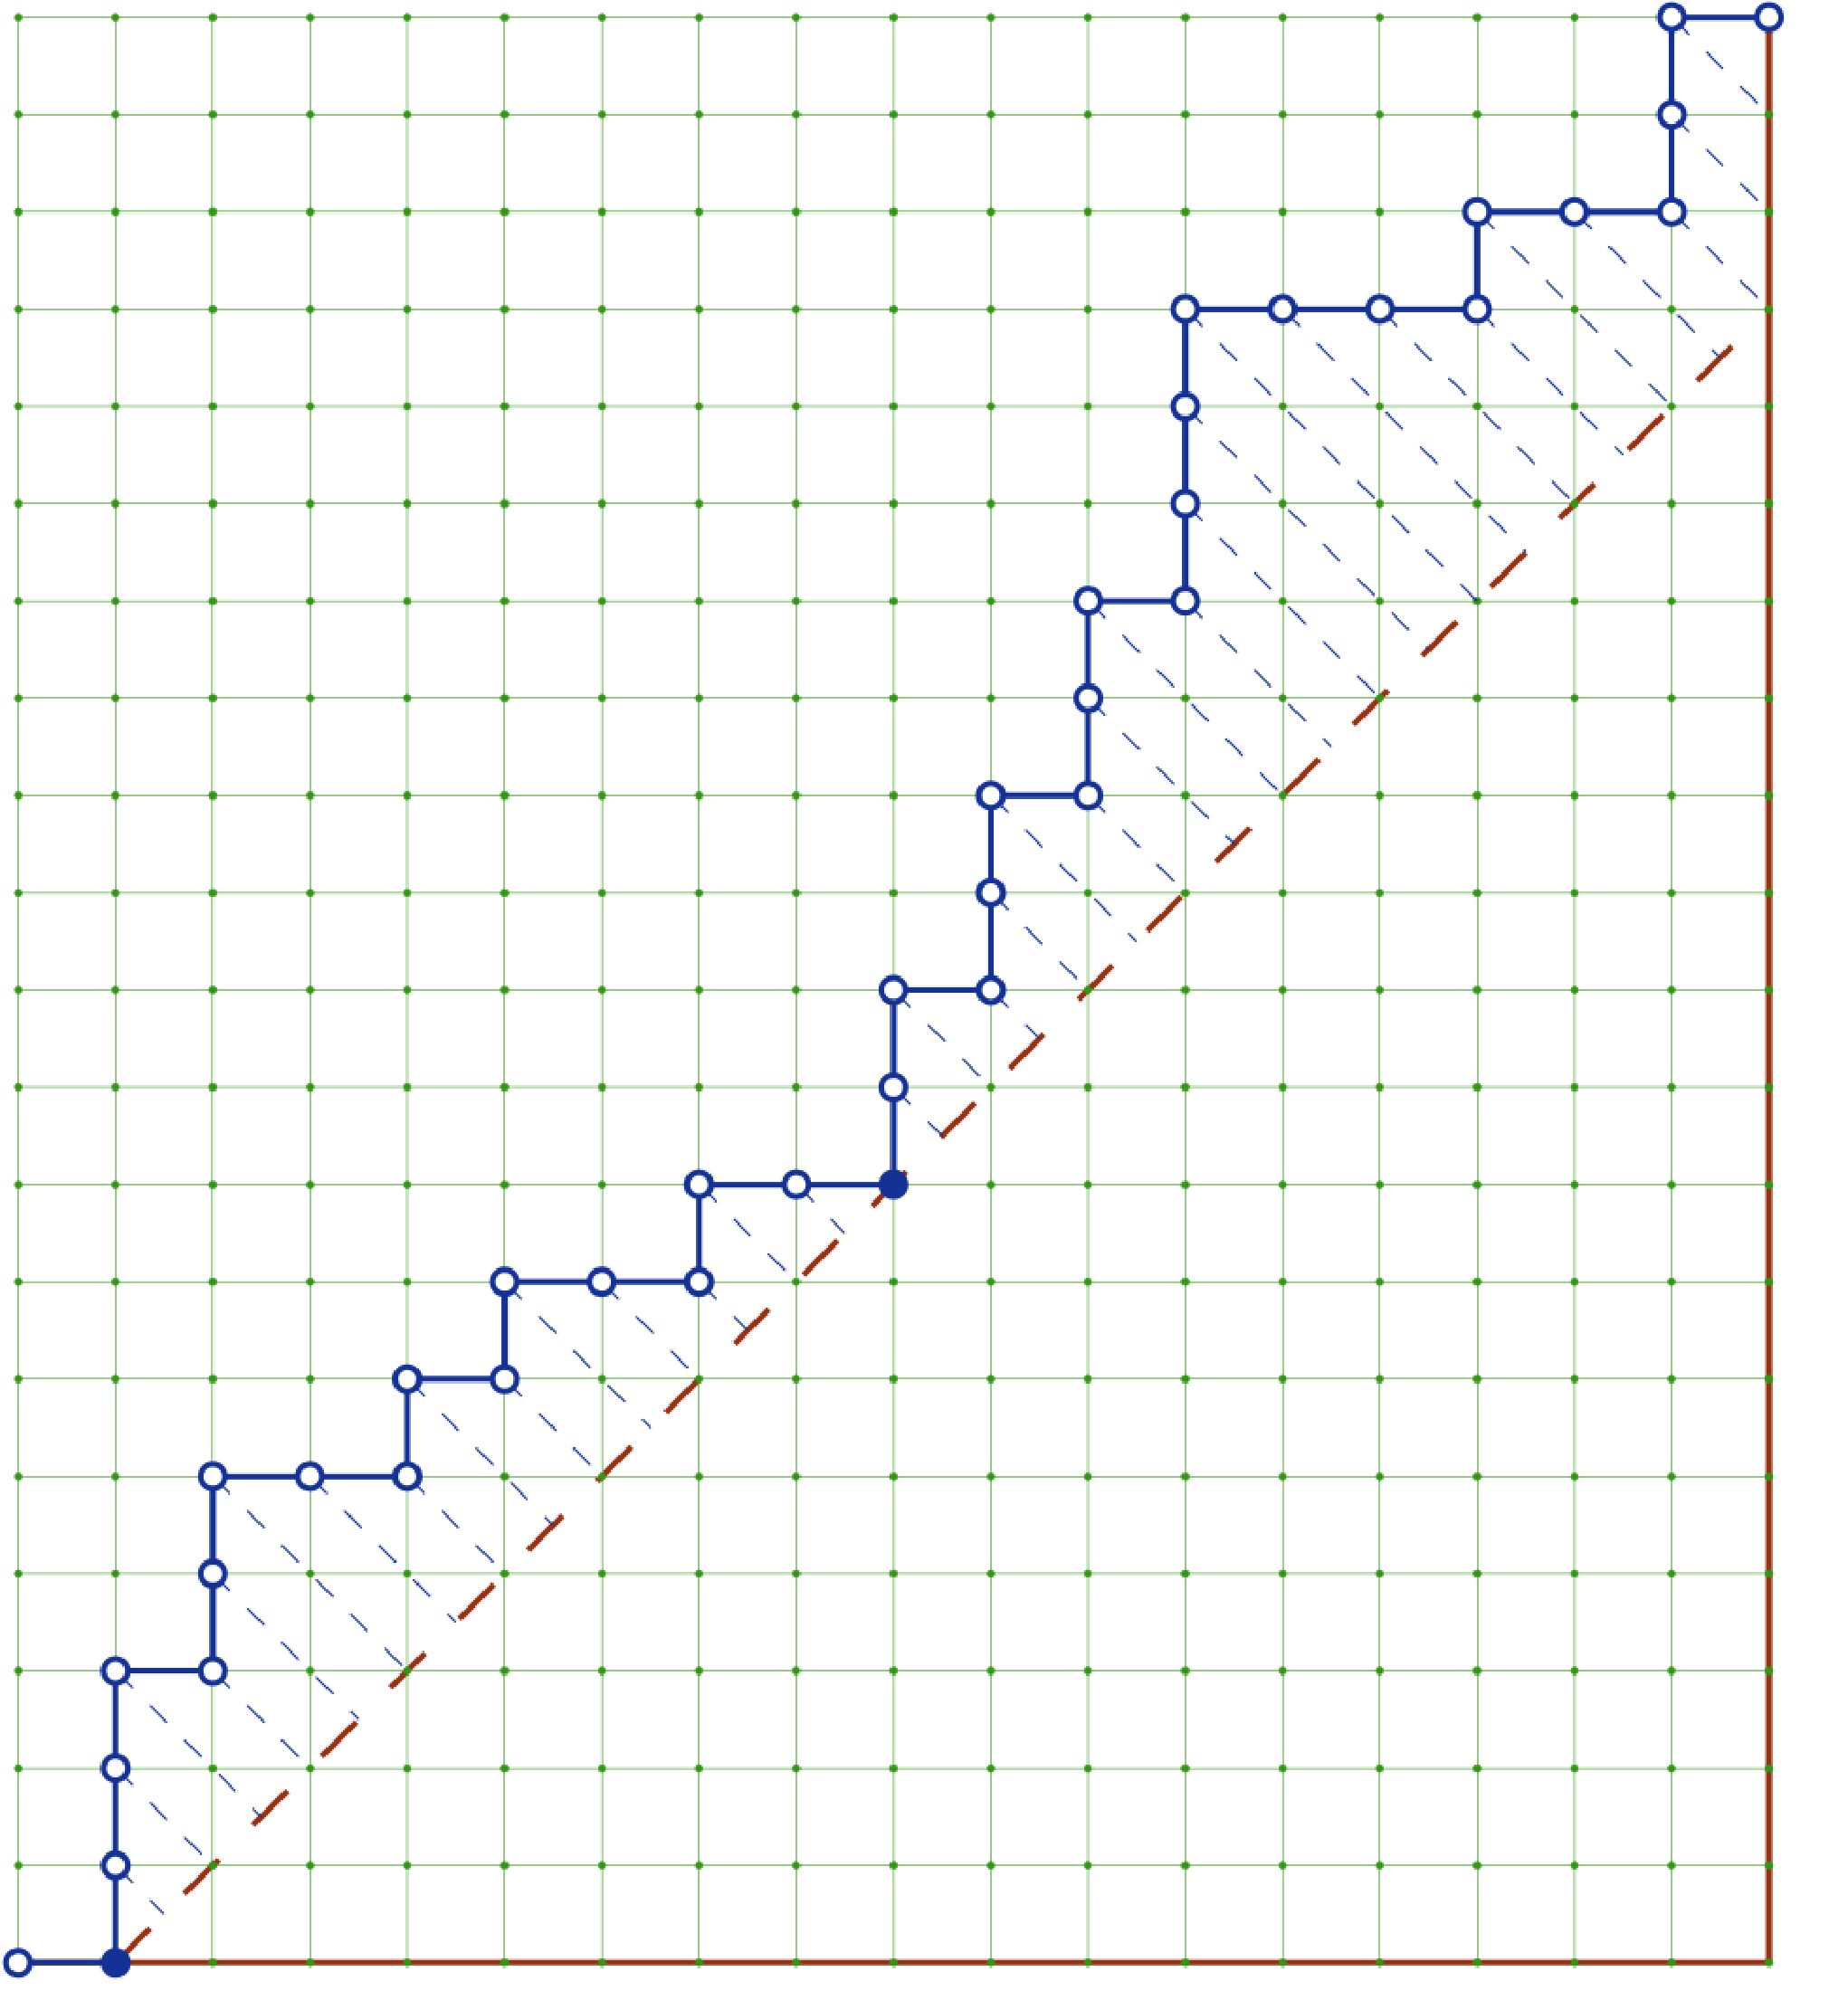
\includegraphics[width=\textwidth]{dyck/complex_dyck_path.pdf}
    \caption{Complex Dyck path with $n = 25$, $m = 22$ and $k = 3$.
             Notice that the boundary is shifted.} \label{fig:complex_dyck}
\end{figure}

\subsection{Generating Dyck Paths}
Our general recursive step is as follows.
We consider a sequence of length $2S$ comprising of $2U$ up moves ($+1$) and $2D$ down moves ($-1$).
Additionally, the sum of any initial sequence {\color{red} prefix?} canon be less than $k-1$.
Without loss of generality, let's assume that $2D\le S$. If this were not the case,
we could simply flip the sequence and negate the elements.
This essentially means that the overall Dyck path is non-decreasing.

\begin{lemma}
$S-2D = \Bo(\log n\sqrt S) \implies U-D = \Bo(\log n\sqrt S)$
\label{lem:dyck_var0}
\end{lemma}

We want to sample the height of this path after $S$ steps.
This is the same as sampling the number of $(+1)$s that get assigned to the first half of the elements in the sequence.
We define $p_d$ as the probability that exactly $D-d$ $(-1)$s get assigned to the first half.
This means that exactly $U+d$ $(+1)$s get assigned to the first half.
Consequently, the second half will contain exactly $D+d$ $(-1)$s and $U-d$ $(+1)$s.
\todo{What is $d$ is negative?}


Let us first compute this probability.
$$
p_d = \frac{D_{left}\cdot D_{right}}{D_{tot}}
$$
Here, $D_{left}$ denotes the number of valid starting sequences (first half)
and $D_{right}$ denotes the number of valid ending sequences.
Here, \textit{valid} means that each half sequence gets the appropriate number of ups and downs
and the initial sums never drop below $1-k$.
For, $D_{right}$, we will start the Dyck path from the end of the $2S$ sequence.
In this case the invalidation threshold will be a different $k'$.
This $k'$ is the final height of the $2S$ sequence. So, $k'=k+2U-2D = k+4S-2D$.
We will use this fact extensively moving forward.

Also, $D_{tot}$ is the total number of possible sequences of length $2S$, given the initial conditions.
Note that in this case the threshold remains at $k$.

We will use the following rejection sampling lemma from \cite{huge}.
\todo{Frequently?}
\begin{lemma}
\label{lem:huge}
Let $\{p_i\}$ and $\{q_i\}$ be distributions satisfying the following conditions
\begin{enumerate}
    \item There is a poly-time algorithm to approximate $p_i$ and $q_i$ up to $\pm n^{-2}$
    \item Generating an index $i$ according to $q_i$ is closely implementable.
    \item There exists a $poly(log n)$-time recognizable set $S$ such that
    \begin{itemize}
        \item $1-\SL{i\in S}{} p_i$ is negligible
        \item There exists a constant $c$ such that for every $i$, it holds that $p_i\le \log^{\mathcal{O}(1)} n\cdot q_i$
    \end{itemize}
\end{enumerate}
Then, generating an index $i$ according to the distribution $\{p_i\}$ is closely-implementable.
\end{lemma}

\begin{algorithm}[H]
    \caption{Na\"{i}ve Generator}
    \begin{algorithmic}
        \Procedure{Split}{$U, D, k$}
            \State{$S \gets U + D$}\\
            \State{$d \sim \left\{\frac{\binom{S}{S-d}\binom{S}{D+d}}{\binom{2S}{2D}}\right\}_d$}\\\\
            \State{$k' \gets k + U - D$}\\
            \State{$p_d \gets
                \frac{{{S}\choose{D-d}}-{{S}\choose{D-d-k}}{{S}\choose{U-d}}
                -{{S}\choose{U-d-k'}}}{{{2S}\choose{2D}}-{{2S}\choose{2D-k}}}$}
            \State{$q_d \gets \frac{\binom{S}{S-d}\binom{S}{D+d}}{\binom{2S}{2D}}$}\\
            \If {$p_d < q_d$}
                \State \Return $d$
            \EndIf
            \State{\textbf{draw} $X \sim\distr{Bern}(p_d/q_d)$}
            \If {$X = 0$}
                \State \Return $d$
            \EndIf
            \Return \func{Split}($U, D, k, k'$)

        \EndProcedure
        \Procedure{Height}{$x$}
            \If {$x\in heights$}
                \State \Return $heights[x]$
            \EndIf
            \State{$l \gets \func{lower-bound}(x)$}
            \State{$r \gets \func{upper-bound}(x)$}
            \State{$h_l \gets \func{Height}(l)$}
            \State{$h_r \gets \func{Height}(r)$}
            \State{$extra \gets (r-l)-(h_r-h_l)$}
            \State{$U\gets (h_r-h_l) + extra/2$}
            \State{$D\gets extra/2$}
            \State{$k\gets 1 + h_l$}
            \State{$d \gets \func{Split}(U,D,k)$}
            \State{$heights[(r+l)/2] \gets h_l + U + d$}
            \State \Return $\func{Height}(x)$
        \EndProcedure
    \end{algorithmic}
    \label{alg:naive}
\end{algorithm}

\input{dyck/height}
\subsection{Supporting ``First Return'' Queries}%
\label{sec:supporting_first_return_queries}

We might want to support more complex queries to a Dyck path.
Specifically, in addition to querying the height of a position,
we might want to know the next time the path return to that height (if at all).
We introduce a new query $\func{First-Return}(x)$ which returns the first time the walk returns to
$\func{Height}(x)$ if the step from $x$ to $x+1$ is an up-step.

The utility of this kind of query can be seen in other interpretations of Catalan objects.
For instance, if we interpret it as a well bracketed expression,
$\func{First-Return}(x)$ returns the position of the bracket matching the one started at $x$.
If we consider a uniformly random rooted tree, the fucntion effectively returns the next child of a vertex.
\todo{Explain why}

We will use the following asymptotic formula for \emph{close-to-central} binomial coefficients.
\begin{restatable}{lemma}{CentralBinomialCoefficients}
\label{lem:CentralBinomialCoefficients}
If $k = \frac{n \pm c\sqrt n}{2}$ where $c = o(n^{1/6})$,
we can approximate $\binom{n}{k}$ up to constant factors by the expression:
\[
\frac{2^n}{\sqrt n}\cdot \mathlarger e^{-c^2/2}
\]
\end{restatable}

We maintain a threshold $\mathcal T = \Theta(\log^7 n)$.
If an un-sampled interval in the Dyck path has length less than $\mathcal T$, then we sample the entire interval.
So, for intervals with length $S > \mathcal T$,
the maximum deviations are bounded by $\mathcal O(\log n\sqrt S) = \mathcal O(\log^{4.5}n)$ with high probability.
Specifically, this means that if we write the deviation as $c\sqrt n$, we see that $c = \log n$ which is $o(S^{1/6})$.
\todo{Formalize this notion of deviations}


\subsubsection{Maintaining a Boundary Invariant}%
\label{sec:maintaining_a_boundary_invariant}
\todo{Why?}
Consider all positions that have been queried already $ \langle x_1, x_2,\cdots, x_m \rangle$ (in increasing order)
along with their corresponding heights $ \langle h_1, h_2,\cdots, h_m \rangle$.
We maintain an invariant that for each $i < m$,
the Dyck path between positions $x_i$ and $x_{i+1}$ is constrained to lie above $min(h_i, h_{i+1})$.
\begin{figure}[htpb]
    \centering
    \includegraphics[width=1.0\linewidth, trim={0 12cm 0 12cm}]{images/dyck_boundary_invariant.pdf}
    \caption{Error in third segment.}
    \label{fig:dyck_boundary_invariant}
\end{figure}

It is not even clear that this is always possible.
After sampling the height of a particular position $x_i$ as $h_i$ (with $x_{i-1} < x_i < x_{i+1}$),
the invariant is potentially broken on either side of $x_i$.
We will re-establish the invariant by sampling an additional point on either side.
This proceeds as follows for the interval between $x_i$ and $x_{i+1}$
(see error in Figure~\ref{fig:dyck_boundary_invariant}):
\begin{enumerate}
    \item Sample the lowest height $h$ achieved by the walk between $x_i$ and $x_{i+1}$.
    \item Sample a position $x$ such that $x_i < x < x_{i+1}$ and $\func{Height}(x) = h$.
\end{enumerate}
Since $h$ is the minimum height along this interval, sampling the point $x$ suffices to preserve the invariant.


\subsubsection{Sampling the Lowest Achievable Height}%
\label{ssub:sampling_the_lowest_achievable_height}
For the first step, we need to sample the lowest height of the walk between $x_i$ and $x_{i+1}$.
Notice that we can assume $x_i < x_{i+1}$ without loss of generality (if $x_i > x_{i+1}$, swap them and proceed).
Let's say that the boundary is currently $k'-1$ units below $h_i$.

We know how to count the numnber of possible Dyck paths for any given boundary.
Dividing by the total number of possible paths gives us precisely the CDF we need.
This allows us to binary search to find the boundary.

We will use $D_{k}$ to denote the number of paths that respect a boundary which is $k-1$ units below $h_i$.
So, in the first step, we compute $p = D_{k'/2}/D_{k'}$.
This means that with probability $p$, the path never reaches height $h_i - k'/2$.
Otherwise, the path must reach $h_i-k'/2$ but not $h_i-k'$.
Note that we can also calculate the total number of such paths as $D_{k'} - D_{k'/2}$.
We repeat this procedure, essentially performing binary search,
until we find a $k$ such that the path reaches height $h_i-k+1$ (potentially multiple times), but never goes below it.


\subsubsection{Sampling the Position of First Return}%
\label{sec:sampling_the_location_of_first_return}
Now that we have a ``\emph{mandatory boundary}'' $k$, we just need to sample a position $x$ with height $h = x_i-k+1$.
In fact, we will do something stronger by sampling the \emph{first} time the walk touches the boundary after $x_i$.
\begin{figure}[htpb]
    \centering
    \includegraphics[width=1.0\linewidth, trim={0 6cm 0 5cm}]{images/dyck_return_sampling.pdf}
    \caption{Zooming into (and flipping) the error in Figure~\ref{fig:dyck_return_sampling}}
    \label{fig:dyck_return_sampling}
\end{figure}

We will parameterize the position $x$ the number of up-steps between $x_i$ and $x$
(See Figure~\ref{fig:dyck_return_sampling}).
This quantity will be referred to as $d$ such that $x - x_{i+1} = 2d + k-1$.
Given a specific $d$, we want to compute the number of valid paths that result in
$d$ up-steps before the first approach to the boundary.
We will calculate this quantity by counting the total number of paths to the left and right
of the first approach and multiplying them together.

Since we only care about getting a asymptotic (up to $\poly(\log n)$ factors) estimate of the probabilities,
it suffices to estimate the number of paths asymptotically as well.

\begin{restatable}{lemma}{ReturnDLeftBound}
\label{lem:ReturnDLeftBound}
If $d > \log^7 n$, then $D_{left}(d)
= \Theta\left( \frac{2^{2d+k}}{\sqrt{d}}\mathlarger e^{-r_{left}(d)}\cdot \frac{k-1}{d+k-1}\right)$
where $r_{left}(d) = \frac{(k-2)^2}{2(2d+k-2)}$.
\end{restatable}
\todo{Deal with smaller values of $d$}

\begin{restatable}{lemma}{ReturnDRightBound}
\label{lem:ReturnDRightBound}
If $U+D-2d-k > \log^7 n$, then $D_{right}(d)
= \Theta\left( \frac{2^{U+D-2d-k}}{\sqrt{U+d-2d-k}}\mathlarger e^{-r_{right}(d)}\cdot \frac{U-D+k}{U-d+1}\right)$
where $r_{right}(d) = \frac{(U-D-k-1)^2}{4(U+D-2d-k+1)}$.
\end{restatable}
\todo{Deal with other values of $d$}


\subsubsection{Estimating the CDF}%
\label{ssub:estimating_the_cdf}

\begin{restatable}{lemma}{ReturnProbabilityBoundNotNormalized}
\label{lem:ReturnProbabilityBoundNotNormalized}
$D_{left}(d)\cdot D_{right}(d)
= \Theta\left( \frac{2^{U+D}}{\sqrt{d(U+D-2d-k)}}\mathlarger e^{-r(d)}\cdot\frac{k-1}{d+k-1}\cdot\frac{U-D+k}{U-d+1}\right)$
where $r(d)=\mathcal O(\log^2 n)$.
\end{restatable}
\begin{proof}
This follows from the fact that both $r_{left}(d)$ and $r_{right}(d)$ are $\mathcal O(\log^2 n)$.
\end{proof}

\begin{corollary}
\label{cor:ReturnProbabilityRounding}
The probability $p_d$ of sampling $d$ as the number of up-steps
before the first approach to the boundary can be approximated as:
\[
p_d = \Theta\left( \frac{ 2^{U+D}\cdot\frac{(k-1)(U-D+k)}{\sqrt{d(U+D-2d-k)}(d+k-1)(U-d+1)}\cdot
\mathlarger e^{-\floor{r(d)}} }{\binom{U+D}{U}-\binom{U+D}{D-k}} \right)
\]
\todo{$D_{total}$ is not correct}
This is because the floor function only affects the value of the exponential by a factor of at most $e$.
\end{corollary}
\begin{corollary}
\label{cor:ReturnProbabilityPiecewiseContinuous}
We define a piecewise continuous function
\[
\hat q(d) = \frac{ 2^{U+D}\cdot\frac{(k-1)(U-D+k)}{\sqrt{d(U+D-2d-k)}(d+k-1)(U-d+1)}\cdot
\mathlarger e^{-\floor{r(d)}} }{\binom{U+D}{U}-\binom{U+D}{D-k}}
\]
We claim that $p_d = \Theta\left( \int\limits_d^{d+1} \hat q(d)\right)$.
Note that this integral has a closed form for a fixed value of $\floor{r(d)}$.
\end{corollary}


Let the maximum value of $r(d)$ be $r_{max} = \mathcal O(\log^2 n)$.
\begin{corollary}
\label{cor:}
We can compute the approximate normalized probabilities
\[
q_d = \frac{\int\limits_d^{d+1} \hat q(d)}{\int\limits_1^{n} \hat q(d)}
\]
such that $p_d = \Theta(q_d)$.
Furthermore, we can also compute the CDF of $q_d$ as:
\[
Q_d = \frac{\int\limits_1^{d+1} \hat q(d)}{\int\limits_1^{n} \hat q(d)}
\]
This allows us to sample from the distribution $q_d$ and use Lemma~\ref{lem:huge} to indirectly sample from $p_d$.
\end{corollary}



